%%%%%%%%%%%%%%%%%%%%%%%%%%%%%%%%%%%%%%%%%
%  My documentation report
%  Objetive: Explain what I did and how, so someone can continue with the investigation
%
% Important note:
% Chapter heading images should have a 2:1 width:height ratio,
% e.g. 920px width and 460px height.
%
%%%%%%%%%%%%%%%%%%%%%%%%%%%%%%%%%%%%%%%%%

%----------------------------------------------------------------------------------------
%	PACKAGES AND OTHER DOCUMENT CONFIGURATIONS
%----------------------------------------------------------------------------------------

\documentclass[11pt,fleqn]{book} % Default font size and left-justified equations

\usepackage[top=3cm,bottom=3cm,left=3.2cm,right=3.2cm,headsep=10pt,letterpaper]{geometry} % Page margins

\usepackage{graphicx}

\usepackage{amssymb}

\usepackage{amsmath}

\usepackage{epstopdf}
\DeclareGraphicsRule{.tif}{png}{.png}{`convert #1 `dirname #1`/`basename #1 .tif`.png}
\DeclareGraphicsRule{.gif}{png}{.png}{`convert #1 `dirname #1`/`basename #1 .gif`.png}

\usepackage[]{nomencl}

\usepackage{float} 

\usepackage{enumitem}

\usepackage{lipsum}

\usepackage{color}

\definecolor{dkgreen}{rgb}{0, 0.6, 0}
\definecolor{gray}{rgb}{0.5, 0.5, 0.5}
\definecolor{mauve}{rgb}{0.58, 0, 0.82}

\usepackage{listings}

\usepackage{wrapfig}

\lstset{
    language=R,
    basicstyle=\footnotesize,
    numbers=left,
    numberstyle=\tiny\color{gray},
    stepnumber=1,
    numbersep=5pt,
    backgroundcolor=\color{white},
    showspaces=false,
    showstringspaces=false,
    showtabs=false,
    frame=tb,
    rulecolor=\color{black},
    tabsize=2,
    captionpos=b,
    breaklines=true,
    breakatwhitespace=false,
    title=\lstname,
    keywordstyle=\color{blue},
    commentstyle=\color{dkgreen},
    stringstyle=\color{mauve},
    escapeinside={\%*}{*)},
    morekeywords={*,...}
}

\usepackage{setspace}

\usepackage{xcolor} % Required for specifying colors by name
\definecolor{ocre}{RGB}{52,177,201} % Define the orange color used for highlighting throughout the book

% Font Settings
\usepackage{avant} % Use the Avantgarde font for headings
%\usepackage{times} % Use the Times font for headings
\usepackage{mathptmx} % Use the Adobe Times Roman as the default text font together with math symbols from the Sym­bol, Chancery and Com­puter Modern fonts

\usepackage{microtype} % Slightly tweak font spacing for aesthetics
\usepackage[utf8]{inputenc} % Required for including letters with accents
\usepackage[T1]{fontenc} % Use 8-bit encoding that has 256 glyphs

% Bibliography
\usepackage[style=alphabetic,sorting=nyt,sortcites=true,autopunct=true,babel=hyphen,hyperref=true,abbreviate=false,backref=true,backend=biber]{biblatex}
\addbibresource{bibliography.bib} % BibTeX bibliography file
\defbibheading{bibempty}{}

%----------------------------------------------------------------------------------------
%	VARIOUS REQUIRED PACKAGES
%----------------------------------------------------------------------------------------

\usepackage{titlesec} % Allows customization of titles

\usepackage{graphicx} % Required for including pictures
\graphicspath{{Pictures/}} % Specifies the directory where pictures are stored

\usepackage{lipsum} % Inserts dummy text

\usepackage{tikz} % Required for drawing custom shapes

\usepackage[english]{babel} % English language/hyphenation

\usepackage{enumitem} % Customize lists
\setlist{nolistsep} % Reduce spacing between bullet points and numbered lists

\usepackage{booktabs} % Required for nicer horizontal rules in tables

\usepackage{eso-pic} % Required for specifying an image background in the title page

%----------------------------------------------------------------------------------------
%	MAIN TABLE OF CONTENTS
%----------------------------------------------------------------------------------------

\usepackage{titletoc} % Required for manipulating the table of contents

\contentsmargin{0cm} % Removes the default margin
% Chapter text styling
\titlecontents{chapter}[1.25cm] % Indentation
{\addvspace{15pt}\large\sffamily\bfseries} % Spacing and font options for chapters
{\color{ocre!60}\contentslabel[\Large\thecontentslabel]{1.25cm}\color{ocre}} % Chapter number
{}  
{\color{ocre!60}\normalsize\sffamily\bfseries\;\titlerule*[.5pc]{.}\;\thecontentspage} % Page number
% Section text styling
\titlecontents{section}[1.25cm] % Indentation
{\addvspace{5pt}\sffamily\bfseries} % Spacing and font options for sections
{\contentslabel[\thecontentslabel]{1.25cm}} % Section number
{}
{\color{black}\sffamily\;\titlerule*[.5pc]{.}\;\thecontentspage} % Page number
[]
% Subsection text styling
\titlecontents{subsection}[1.25cm] % Indentation
{\addvspace{1pt}\sffamily\small} % Spacing and font options for subsections
{\contentslabel[\thecontentslabel]{1.25cm}} % Subsection number
{}
{\sffamily\;\titlerule*[.5pc]{.}\;\thecontentspage} % Page number
[] 

%----------------------------------------------------------------------------------------
%	MINI TABLE OF CONTENTS IN CHAPTER HEADS
%----------------------------------------------------------------------------------------

% Section text styling
\titlecontents{lsection}[0em] % Indendating
{\footnotesize\sffamily} % Font settings
{}
{}
{}

% Subsection text styling
\titlecontents{lsubsection}[.5em] % Indentation
{\normalfont\footnotesize\sffamily} % Font settings
{}
{}
{}
 
%----------------------------------------------------------------------------------------
%	PAGE HEADERS
%----------------------------------------------------------------------------------------

\usepackage{fancyhdr} % Required for header and footer configuration

\pagestyle{fancy}
\renewcommand{\chaptermark}[1]{\markboth{\sffamily\normalsize\bfseries\chaptername\ \thechapter.\ #1}{}} % Chapter text font settings
\renewcommand{\sectionmark}[1]{\markright{\sffamily\normalsize\thesection\hspace{5pt}#1}{}} % Section text font settings
\fancyhf{} \fancyhead[LE,RO]{\sffamily\normalsize\thepage} % Font setting for the page number in the header
\fancyhead[LO]{\rightmark} % Print the nearest section name on the left side of odd pages
\fancyhead[RE]{\leftmark} % Print the current chapter name on the right side of even pages
\renewcommand{\headrulewidth}{0.5pt} % Width of the rule under the header
\addtolength{\headheight}{2.5pt} % Increase the spacing around the header slightly
\renewcommand{\footrulewidth}{0pt} % Removes the rule in the footer
\fancypagestyle{plain}{\fancyhead{}\renewcommand{\headrulewidth}{0pt}} % Style for when a plain pagestyle is specified

% Removes the header from odd empty pages at the end of chapters
\makeatletter
\renewcommand{\cleardoublepage}{
\clearpage\ifodd\c@page\else
\hbox{}
\vspace*{\fill}
\thispagestyle{empty}
\newpage
\fi}

%----------------------------------------------------------------------------------------
%	THEOREM STYLES
%----------------------------------------------------------------------------------------

\usepackage{amsmath,amsfonts,amssymb,amsthm} % For math equations, theorems, symbols, etc

\newcommand{\intoo}[2]{\mathopen{]}#1\,;#2\mathclose{[}}
\newcommand{\ud}{\mathop{\mathrm{{}d}}\mathopen{}}
\newcommand{\intff}[2]{\mathopen{[}#1\,;#2\mathclose{]}}
\newtheorem{notation}{Notation}[chapter]

%%%%%%%%%%%%%%%%%%%%%%%%%%%%%%%%%%%%%%%%%%%%%%%%%%%%%%%%%%%%%%%%%%%%%%%%%%%
%%%%%%%%%%%%%%%%%%%% dedicated to boxed/framed environements %%%%%%%%%%%%%%
%%%%%%%%%%%%%%%%%%%%%%%%%%%%%%%%%%%%%%%%%%%%%%%%%%%%%%%%%%%%%%%%%%%%%%%%%%%
\newtheoremstyle{ocrenumbox}% % Theorem style name
{0pt}% Space above
{0pt}% Space below
{\normalfont}% % Body font
{}% Indent amount
{\small\bf\sffamily\color{ocre}}% % Theorem head font
{\;}% Punctuation after theorem head
{0.25em}% Space after theorem head
{\small\sffamily\color{ocre}\thmname{#1}\nobreakspace\thmnumber{\@ifnotempty{#1}{}\@upn{#2}}% Theorem text (e.g. Theorem 2.1)
\thmnote{\nobreakspace\the\thm@notefont\sffamily\bfseries\color{black}---\nobreakspace#3.}} % Optional theorem note
\renewcommand{\qedsymbol}{$\blacksquare$}% Optional qed square

\newtheoremstyle{blacknumex}% Theorem style name
{5pt}% Space above
{5pt}% Space below
{\normalfont}% Body font
{} % Indent amount
{\small\bf\sffamily}% Theorem head font
{\;}% Punctuation after theorem head
{0.25em}% Space after theorem head
{\small\sffamily{\tiny\ensuremath{\blacksquare}}\nobreakspace\thmname{#1}\nobreakspace\thmnumber{\@ifnotempty{#1}{}\@upn{#2}}% Theorem text (e.g. Theorem 2.1)
\thmnote{\nobreakspace\the\thm@notefont\sffamily\bfseries---\nobreakspace#3.}}% Optional theorem note

\newtheoremstyle{blacknumbox} % Theorem style name
{0pt}% Space above
{0pt}% Space below
{\normalfont}% Body font
{}% Indent amount
{\small\bf\sffamily}% Theorem head font
{\;}% Punctuation after theorem head
{0.25em}% Space after theorem head
{\small\sffamily\thmname{#1}\nobreakspace\thmnumber{\@ifnotempty{#1}{}\@upn{#2}}% Theorem text (e.g. Theorem 2.1)
\thmnote{\nobreakspace\the\thm@notefont\sffamily\bfseries---\nobreakspace#3.}}% Optional theorem note

%%%%%%%%%%%%%%%%%%%%%%%%%%%%%%%%%%%%%%%%%%%%%%%%%%%%%%%%%%%%%%%%%%%%%%%%%%%
%%%%%%%%%%%%% dedicated to non-boxed/non-framed environements %%%%%%%%%%%%%
%%%%%%%%%%%%%%%%%%%%%%%%%%%%%%%%%%%%%%%%%%%%%%%%%%%%%%%%%%%%%%%%%%%%%%%%%%%
\newtheoremstyle{ocrenum}% % Theorem style name
{5pt}% Space above
{5pt}% Space below
{\normalfont}% % Body font
{}% Indent amount
{\small\bf\sffamily\color{ocre}}% % Theorem head font
{\;}% Punctuation after theorem head
{0.25em}% Space after theorem head
{\small\sffamily\color{ocre}\thmname{#1}\nobreakspace\thmnumber{\@ifnotempty{#1}{}\@upn{#2}}% Theorem text (e.g. Theorem 2.1)
\thmnote{\nobreakspace\the\thm@notefont\sffamily\bfseries\color{black}---\nobreakspace#3.}} % Optional theorem note
\renewcommand{\qedsymbol}{$\blacksquare$}% Optional qed square
\makeatother

% Defines the theorem text style for each type of theorem to one of the three styles above
\newcounter{dummy} 
\numberwithin{dummy}{section}
\theoremstyle{ocrenumbox}
\newtheorem{theoremeT}[dummy]{Theorem}
\newtheorem{problem}{Problem}[chapter]
\newtheorem{exerciseT}{Exercise}[chapter]
\theoremstyle{blacknumex}
\newtheorem{exampleT}{Example}[chapter]
\theoremstyle{blacknumbox}
\newtheorem{vocabulary}{Vocabulary}[chapter]
\newtheorem{definitionT}{Definition}[section]
\newtheorem{corollaryT}[dummy]{Corollary}
\theoremstyle{ocrenum}
\newtheorem{proposition}[dummy]{Proposition}

%----------------------------------------------------------------------------------------
%	DEFINITION OF COLORED BOXES
%----------------------------------------------------------------------------------------

\RequirePackage[framemethod=default]{mdframed} % Required for creating the theorem, definition, exercise and corollary boxes

% Theorem box
\newmdenv[skipabove=7pt,
skipbelow=7pt,
backgroundcolor=black!5,
linecolor=ocre,
innerleftmargin=5pt,
innerrightmargin=5pt,
innertopmargin=5pt,
leftmargin=0cm,
rightmargin=0cm,
innerbottommargin=5pt]{tBox}

% Exercise box	  
\newmdenv[skipabove=7pt,
skipbelow=7pt,
rightline=false,
leftline=true,
topline=false,
bottomline=false,
backgroundcolor=ocre!10,
linecolor=ocre,
innerleftmargin=5pt,
innerrightmargin=5pt,
innertopmargin=5pt,
innerbottommargin=5pt,
leftmargin=0cm,
rightmargin=0cm,
linewidth=4pt]{eBox}	

% Definition box
\newmdenv[skipabove=7pt,
skipbelow=7pt,
rightline=false,
leftline=true,
topline=false,
bottomline=false,
linecolor=ocre,
innerleftmargin=5pt,
innerrightmargin=5pt,
innertopmargin=0pt,
leftmargin=0cm,
rightmargin=0cm,
linewidth=4pt,
innerbottommargin=0pt]{dBox}	

% Corollary box
\newmdenv[skipabove=7pt,
skipbelow=7pt,
rightline=false,
leftline=true,
topline=false,
bottomline=false,
linecolor=gray,
backgroundcolor=black!5,
innerleftmargin=5pt,
innerrightmargin=5pt,
innertopmargin=5pt,
leftmargin=0cm,
rightmargin=0cm,
linewidth=4pt,
innerbottommargin=5pt]{cBox}

% Creates an environment for each type of theorem and assigns it a theorem text style from the "Theorem Styles" section above and a colored box from above
\newenvironment{theorem}{\begin{tBox}\begin{theoremeT}}{\end{theoremeT}\end{tBox}}
\newenvironment{exercise}{\begin{eBox}\begin{exerciseT}}{\hfill{\color{ocre}\tiny\ensuremath{\blacksquare}}\end{exerciseT}\end{eBox}}				  
\newenvironment{definition}{\begin{dBox}\begin{definitionT}}{\end{definitionT}\end{dBox}}	
\newenvironment{example}{\begin{exampleT}}{\hfill{\tiny\ensuremath{\blacksquare}}\end{exampleT}}		
\newenvironment{corollary}{\begin{cBox}\begin{corollaryT}}{\end{corollaryT}\end{cBox}}	

%----------------------------------------------------------------------------------------
%	REMARK ENVIRONMENT
%----------------------------------------------------------------------------------------

\newenvironment{remark}{\par\vspace{10pt}\small % Vertical white space above the remark and smaller font size
\begin{list}{}{
\leftmargin=35pt % Indentation on the left
\rightmargin=25pt}\item\ignorespaces % Indentation on the right
\makebox[-2.5pt]{\begin{tikzpicture}[overlay]
\node[draw=ocre!60,line width=1pt,circle,fill=ocre!25,font=\sffamily\bfseries,inner sep=2pt,outer sep=0pt] at (-15pt,0pt){\textcolor{ocre}{R}};\end{tikzpicture}} % Orange R in a circle
\advance\baselineskip -1pt}{\end{list}\vskip5pt} % Tighter line spacing and white space after remark

%----------------------------------------------------------------------------------------
%	SECTION NUMBERING IN THE MARGIN
%----------------------------------------------------------------------------------------

\makeatletter
\renewcommand{\@seccntformat}[1]{\llap{\textcolor{ocre}{\csname the#1\endcsname}\hspace{1em}}}                    
\renewcommand{\section}{\@startsection{section}{1}{\z@}
{-4ex \@plus -1ex \@minus -.4ex}
{1ex \@plus.2ex }
{\normalfont\large\sffamily\bfseries}}
\renewcommand{\subsection}{\@startsection {subsection}{2}{\z@}
{-3ex \@plus -0.1ex \@minus -.4ex}
{0.5ex \@plus.2ex }
{\normalfont\sffamily\bfseries}}
\renewcommand{\subsubsection}{\@startsection {subsubsection}{3}{\z@}
{-2ex \@plus -0.1ex \@minus -.2ex}
{.2ex \@plus.2ex }
{\normalfont\small\sffamily\bfseries}}                        
\renewcommand\paragraph{\@startsection{paragraph}{4}{\z@}
{-2ex \@plus-.2ex \@minus .2ex}
{.1ex}
{\normalfont\small\sffamily\bfseries}}

%----------------------------------------------------------------------------------------
%	HYPERLINKS IN THE DOCUMENTS
%----------------------------------------------------------------------------------------

% For an unclear reason, the package should be loaded now and not later
\usepackage{hyperref}
%\hypersetup{hidelinks,backref=true,pagebackref=true,hyperindex=true,colorlinks=false,breaklinks=true,urlcolor= ocre,bookmarks=true,bookmarksopen=false,pdftitle={Title},pdfauthor={Author}}

%----------------------------------------------------------------------------------------
%	CHAPTER HEADINGS
%----------------------------------------------------------------------------------------

% The set-up below should be (sadly) manually adapted to the overall margin page septup controlled by the geometry package loaded in the main.tex document.
%It is possible to implement below the dimensions used in the goemetry package (top,bottom,left,right)... TO BE DONE

\newcommand{\thechapterimage}{}
\newcommand{\chapterimage}[1]{\renewcommand{\thechapterimage}{#1}}

% Numbered chapters with mini tableofcontents
\def\thechapter{\arabic{chapter}}
\def\@makechapterhead#1{
\thispagestyle{empty}
{\centering \normalfont\sffamily
\ifnum \c@secnumdepth >\m@ne
\if@mainmatter
\startcontents
\begin{tikzpicture}[remember picture,overlay]
\node at (current page.north west)
{\begin{tikzpicture}[remember picture,overlay]
\node[anchor=north west,inner sep=0pt] at (0,0) {\includegraphics[width=\paperwidth]{\thechapterimage}};
%%%%%%%%%%%%%%%%%%%%%%%%%%%%%%%%%%%%%%%%%%%%%%%%%%%%%%%%%%%%%%%%%%%%%%%%%%%%%%%%%%%%%
% Commenting the 3 lines below removes the small contents box in the chapter heading
%\fill[color=ocre!10!white,opacity=.6] (1cm,0) rectangle (8cm,-7cm);
%\node[anchor=north west] at (1.1cm,.35cm) {\parbox[t][8cm][t]{6.5cm}{\huge\bfseries\flushleft \printcontents{l}{1}{\setcounter{tocdepth}{2}}}};
\draw[anchor=west] (6cm,-6.5cm) node [rounded corners=20pt,fill=ocre!10!white,text opacity=1,draw=ocre,draw opacity=1,line width=1.5pt,fill opacity=.6,inner sep=12pt]{\huge\sffamily\bfseries\textcolor{black}{\thechapter. #1\strut\makebox[22cm]{}}};
%%%%%%%%%%%%%%%%%%%%%%%%%%%%%%%%%%%%%%%%%%%%%%%%%%%%%%%%%%%%%%%%%%%%%%%%%%%%%%%%%%%%%
\end{tikzpicture}};
\end{tikzpicture}}
\par\vspace*{200\p@}%Edited vertical spacing within TikZ picture to account for incorrect image Size -GY
\fi
\fi}

% Unnumbered chapters without mini tableofcontents (could be added though) 
\def\@makeschapterhead#1{
\thispagestyle{empty}
{\centering \normalfont\sffamily
\ifnum \c@secnumdepth >\m@ne
\if@mainmatter
\begin{tikzpicture}[remember picture,overlay]
\node at (current page.north west)
{\begin{tikzpicture}[remember picture,overlay]
\node[anchor=north west,inner sep=0pt] at (0,0) {\includegraphics[width=\paperwidth]{\thechapterimage}};
\draw[anchor=west] (6cm,-6.5cm) node [rounded corners=20pt,fill=ocre!10!white,fill opacity=.6,inner sep=12pt,text opacity=1,draw=ocre,draw opacity=1,line width=1.5pt]{\huge\sffamily\bfseries\textcolor{black}{#1\strut\makebox[22cm]{}}};
\end{tikzpicture}};
\end{tikzpicture}}
\par\vspace*{200\p@}%edited vertical spacing here as well to account for unnumbered chapters
\fi
\fi
}
\makeatother
 % Insert the commands.tex file which contains the majority of the structure behind the template

\begin{document}

%----------------------------------------------------------------------------------------
%	TITLE PAGE
%----------------------------------------------------------------------------------------

\begingroup
\thispagestyle{empty}
\AddToShipoutPicture*{\put(0,0){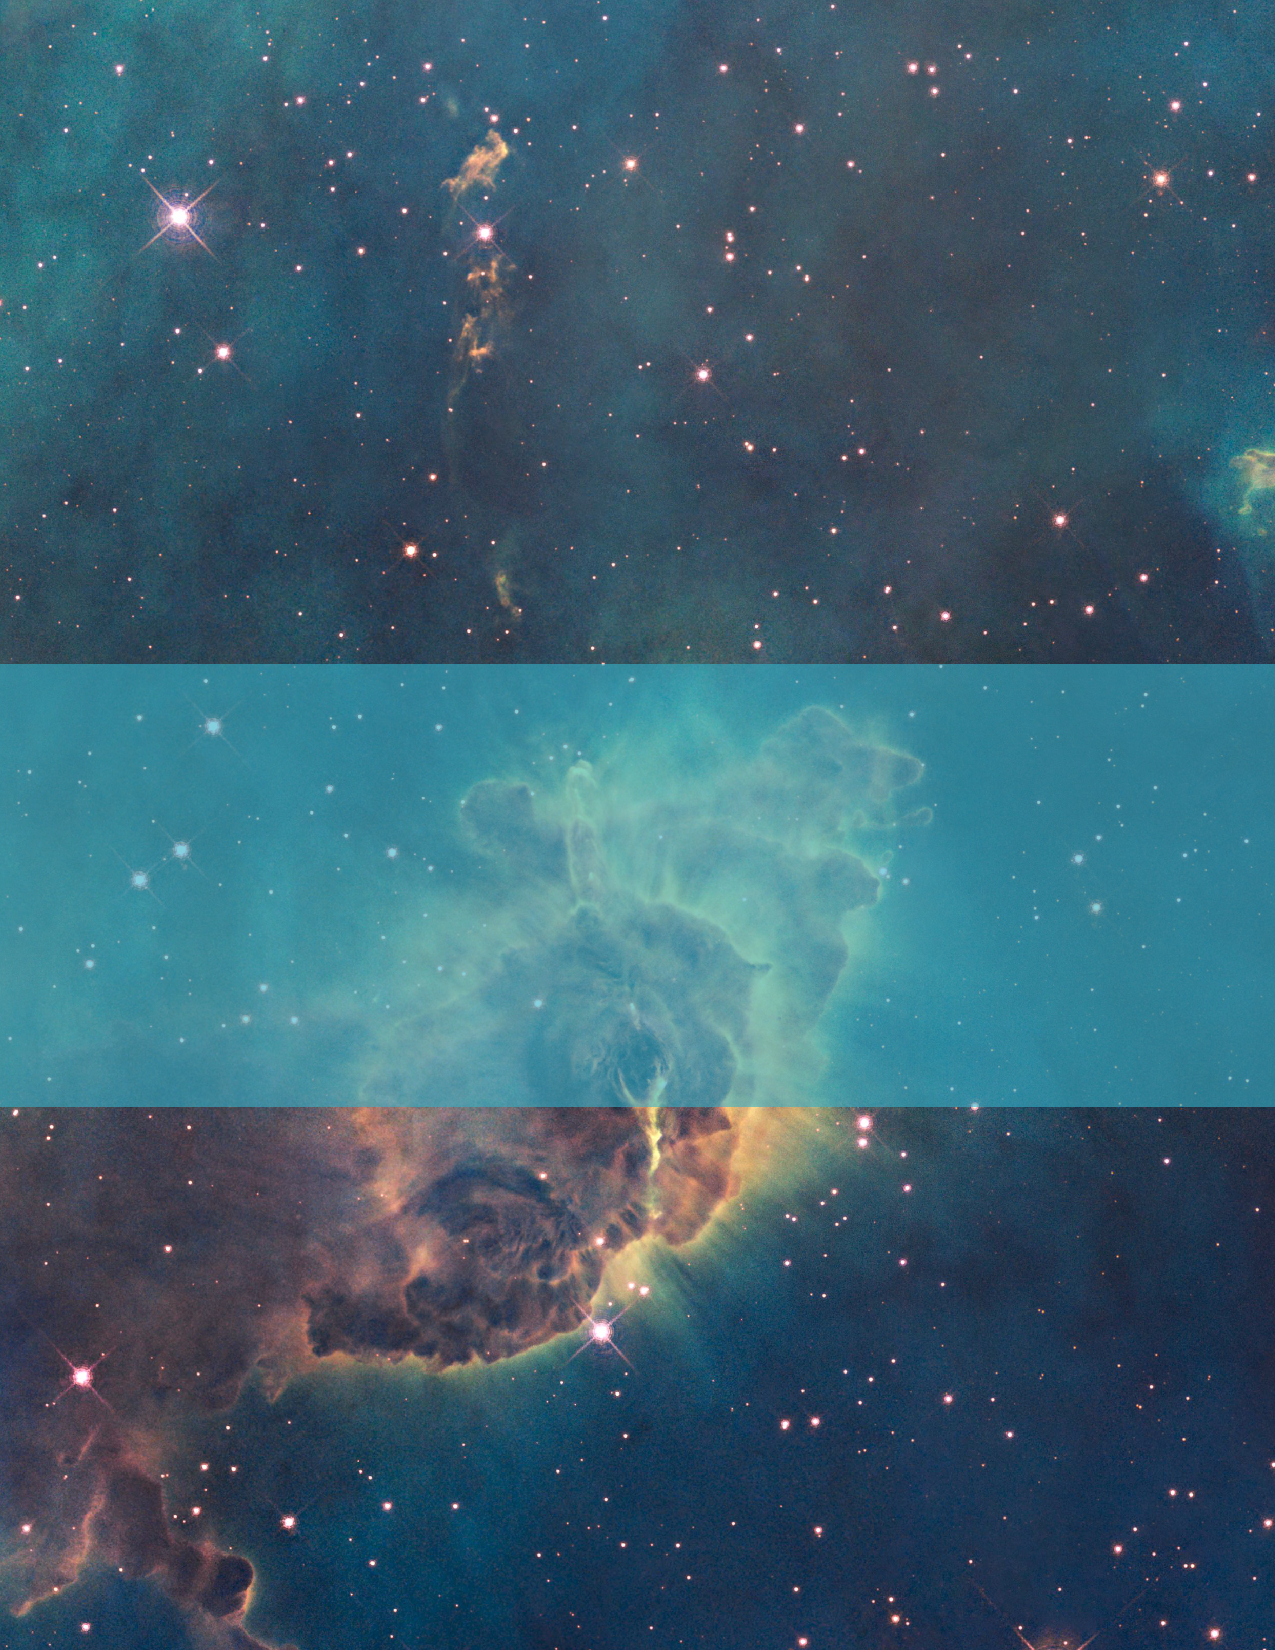
\includegraphics[scale=1.25]{esahubble}}} % Image background
%\AddToShipoutPicture*{\put(0,0){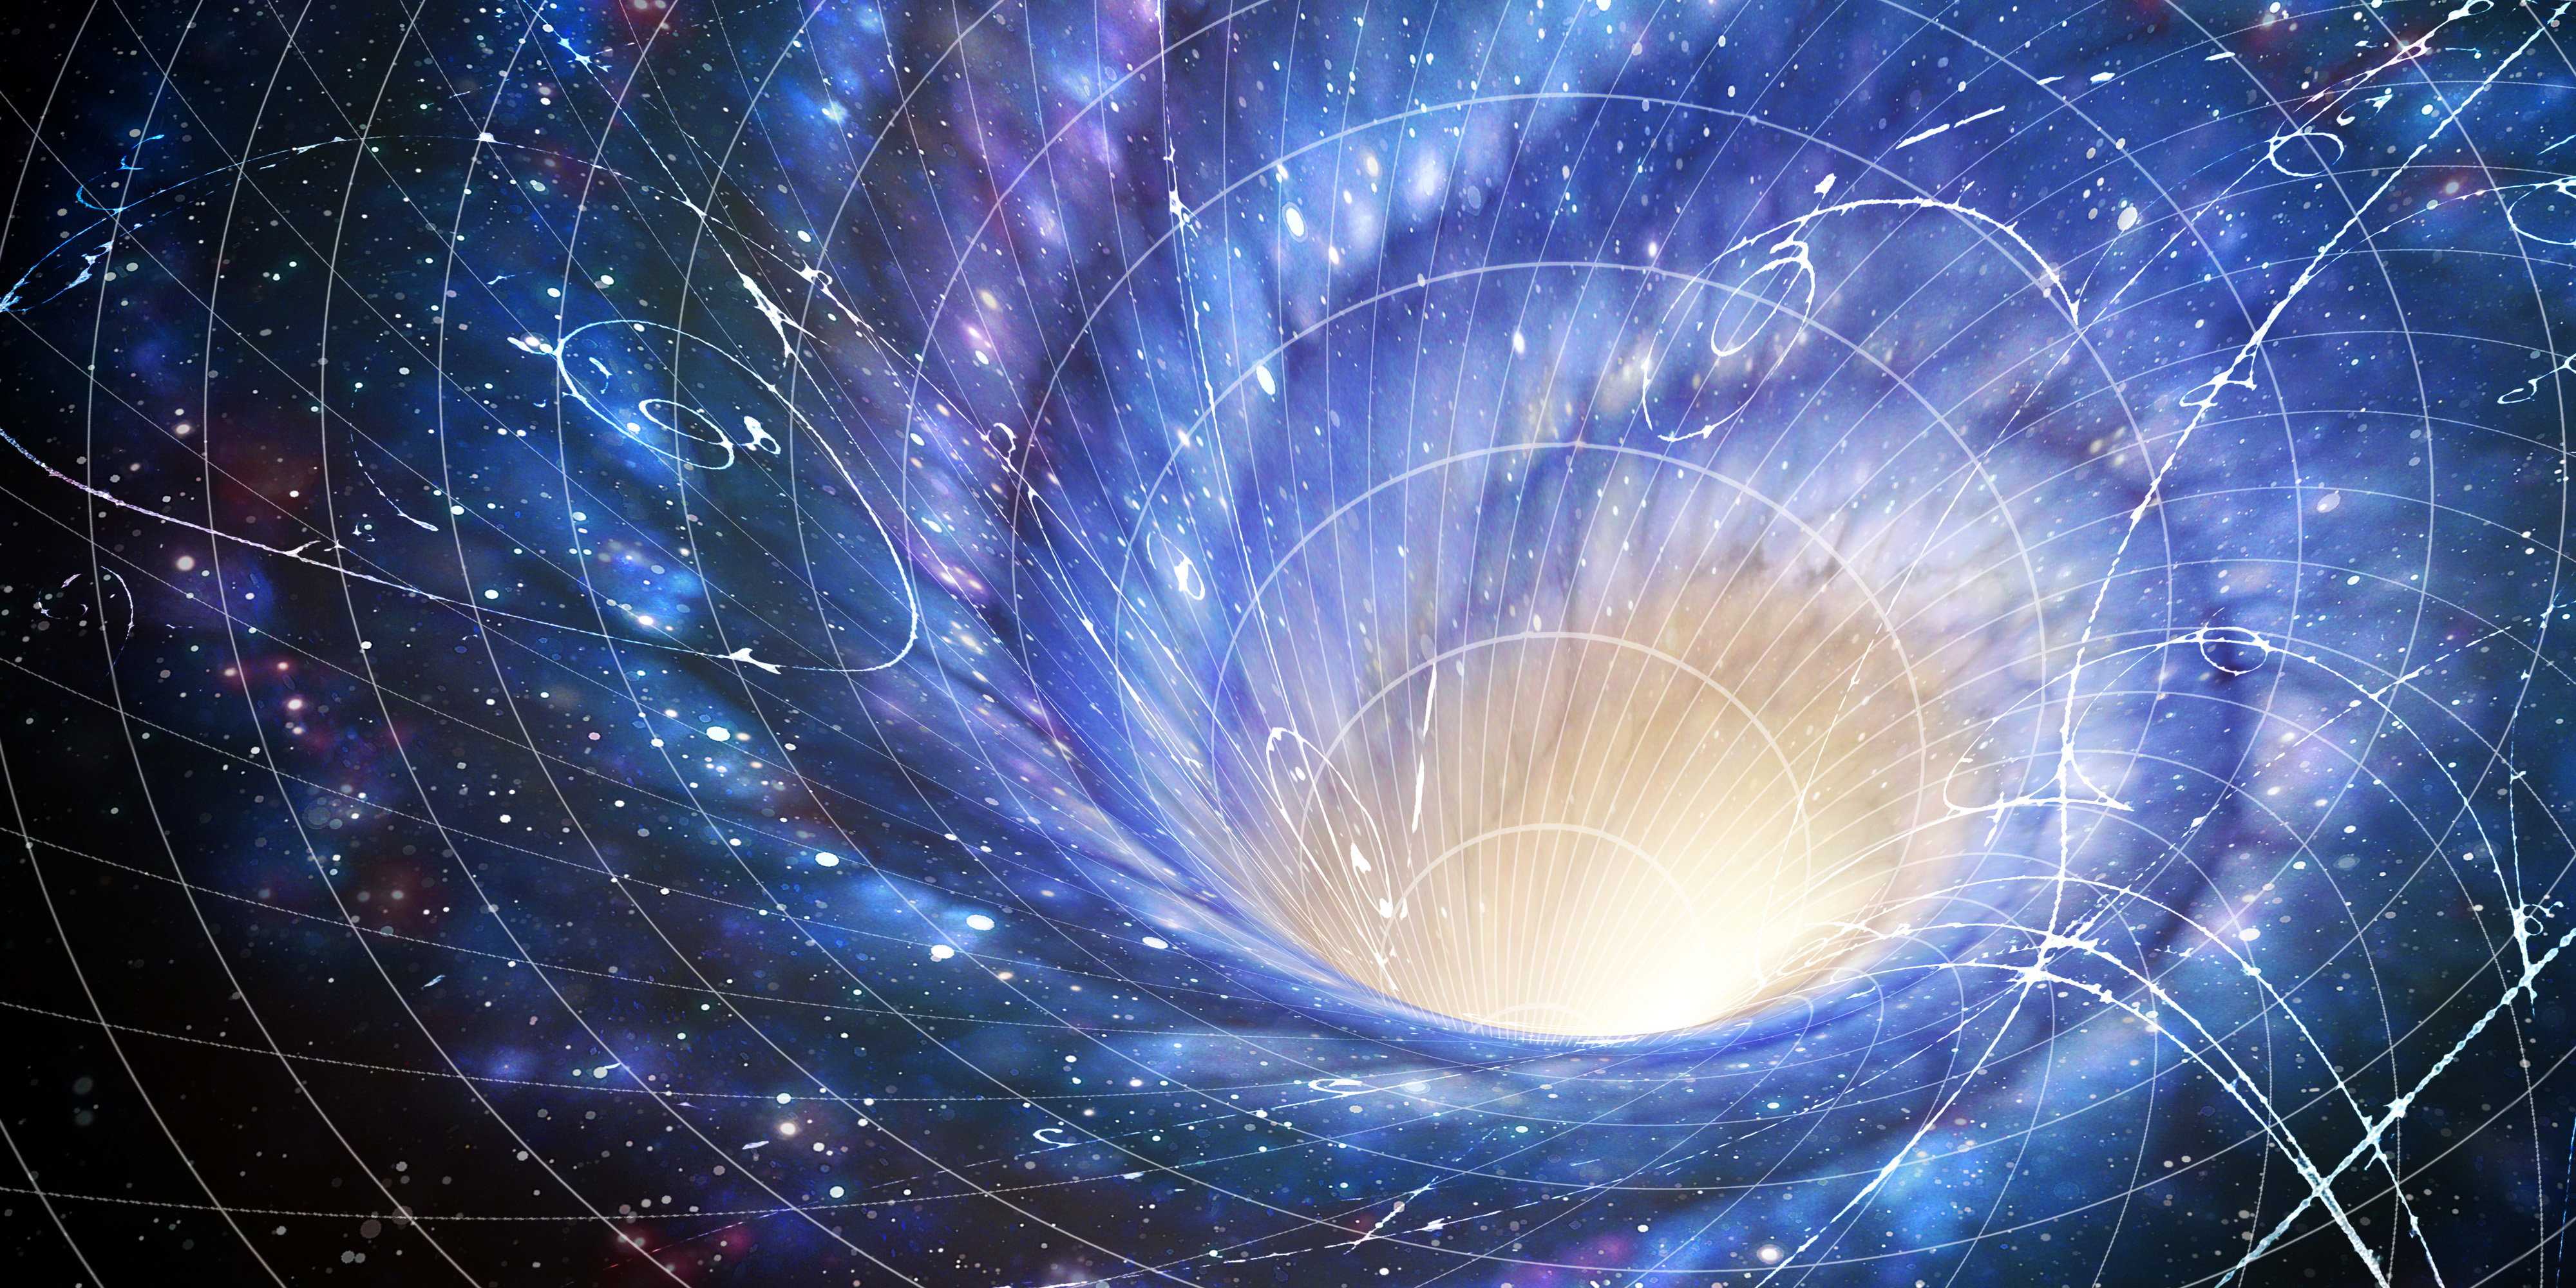
\includegraphics[scale=1.0]{galaxy_spacewarp.jpg}}}
\centering
\vspace*{5cm}
\par\normalfont\fontsize{35}{35}\sffamily\selectfont
\textbf{Case Studies using the R Programming Language}\\
{\LARGE }\par % Book title
\vspace*{1cm}
{\Large Katherine~Bennett, Miguel~de~los~Reyes, Raymond~Gao, Sophia~Hurr, Hannah~Gahagan, Nikhil~Miland, Mridu~Nanda, Christa~Parrish, Ishaan~Rao, Grayson~York }\par % Author name
\endgroup

%----------------------------------------------------------------------------------------
%	COPYRIGHT PAGE
%----------------------------------------------------------------------------------------

\newpage
~\vfill
\thispagestyle{empty}

%\noindent Copyright \copyright\ 2014 Andrea Hidalgo\\ % Copyright notice

\noindent \textsc{Research in Computational Science}\\

\noindent \textsc{North Carolina School of Science and Mathematics, Durham, NC}\\ % URL

\noindent This case studies manual was prepared under the direction of Mr. Robert Gotwals, faculty mentor, The North Carolina School of Science and Mathematics, Durham NC.  \\ % License information

\noindent \textit{First release, November 2016} % Printing/edition date

%----------------------------------------------------------------------------------------
%	TABLE OF CONTENTS
%----------------------------------------------------------------------------------------

\chapterimage{galaxy_spacewarp.jpg} % Table of contents heading image

\pagestyle{empty} % No headers

\tableofcontents % Print the table of contents itself

%\cleardoublepage % Forces the first chapter to start on an odd page so it's on the right

\pagestyle{fancy} % Print headers again

%----------------------------------------------------------------------------------------
%	CHAPTER 1
%----------------------------------------------------------------------------------------

\chapterimage{galaxy_spacewarp.jpg} % Chapter heading image

\chapter{Introduction}

Gotwals will write an Intro.

%  CONTINUING MODIFIABLE STUFF
\chapter{ANOVA}
\section{Introductory Reading}

\nomenclature{Glossary term:}{Definition}

The most common type of linear models are analysis of variance (ANOVA) and linear regression models. 
R is built to handle linear models, and as such it is easy to work with ANOVA. 
ANOVA is a statistical method used to compare two or more means. 
These values can be used to determine whether a significant correlation exists between variables. 
We will be using one-way ANOVA, which compares the means between the groups of interest, and determines whether those means are significantly different from each other. 
If one-way ANOVA returns a significant result, there are at least two group means that are significantly different from each other. 
It is important to note that ANOVA is an omnibus test statistic, meaning that although ANOVA tells the user is there is a significant difference in means, it is unable to show which means in particular differ.
ANOVA can only be used with certain types of data configurations. 
To perform ANOVA, data must have a continuous response variable and at least one categorical factor with two or more levels, in lay terms, ANOVA can only be used with numeric values that can be ordered sequentially, with a certain number of possible responses. 
(i.e. data comparing object's weights, and each new weight is a level) 
ANOVA is easier to use if data is from from approximately normally distributed populations with equal variances between factor levels, however, as R is built to work with statistics, ANOVA procedures will generally work without incident unless one or more of the distributions or variances are highly skewed.
A basic understanding of statistics how to use R is recommended before performing ANOVA. The ANOVA user will create and order factors, make box plots, and combine and stack data. 
\cite{CRANR}
The following functions will be useful in using ANOVA.
\begin{enumerate}
        \item \texttt{aov}
        \item \texttt{as.factor}
        \item \texttt{ls.str}
        \item \texttt{data.frame}
        \item \texttt{stack}
        \item \texttt{TukeyHSD}
\item \texttt{levels}
\end{enumerate}

\section{Objectives}

In this assignment, we will use ANOVA to analyze data from ELISA HIV Optical Density Readings.
ANOVA identifies the causes of variation, and sorts out the corresponding components of variation with associated degrees of freedom. 
In this case, we are interested in seeing how HIV Optical Density Readings are related to their lot. 
The type of ANOVA we are using is one-way between groups, as we are comparing one grouping (the optical density readings) to define the groups (lots). 
\setlist{before=\singlespacing,after=\singlespacing}
\singlespacing
By the end of this lesson, the reader should be able to:
\begin{enumerate}
        \item Understand the logic behind one-way analysis of variance.
        \item Perform one-way analysis of variance in R for any data. 
        \item Appropriately interpret results of analysis of variance tests.
\end{enumerate}

\subsection{ANOVA}

We will look at variances in data using R's ANOVA functions.

\subsection{Visualization}

We will also use our fitted models and our ANOVA data to create box plots and line plots.
Much of the information gleaned from ANOVA is presented via numeric such as the sum of square, degrees of freedom, and the mean.
ANOVA presents the null hypothesis that there is no difference in means of the treatments, and once this hypothesis is proven incorrect, the question arises of how the treatments differ.
The post-hoc test also allows the user to find the differences in means, and specifically categorizes the lower and upper means of the data.

Figure \ref{fig:BoxPlotOpticalDensity} shows a box plot of the data before running ANOVA or TukeyHSD.
Constructing a box plot before analyzing the data may prove helpful in deciding what kind of analysis would be preferable.

\begin{figure}%  the "H" means put it where you put this code....but that doesn't always work!
        \centering
                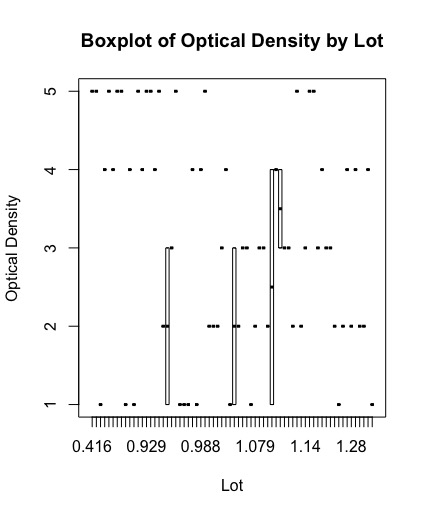
\includegraphics[width = .5\textwidth]{pictures/ANOVA/BoxPlotOpticalDensity.jpg} 
        \caption{Boxplot}
        \label{fig:BoxPlotOpticalDensity}
\end{figure}

 

\section{Building the Model}

Looking at the data set of interest for ANOVA, note that that data may be in numeric form. Use the function is.numeric to review the data. If this function prints TRUE, use the function as.factor to change data from numeric to factor. In order to make it easier to manipulate data later on, it is recommended that the factored data is renamed. 
\begin{lstlisting}
lot = as.factor(elisa$Lot)
summary(lot)
levels(as.factor(elisaOptical))
optical = (as.factor(elisa$Optical))
levels(as.factor(elisa$Run))
run = (as.factor(elisa$Run))
\end{lstlisting}
Now your factor data type is in non-numerical variables.
Each different variable of the factor is called a level.
For example, our factor type data for the lots of various ELISA HIV Optical Density Readings has five levels, 1, 2, 3, 4 and 5.
Moving on, we can make a box plot of our data, so that we can visually compare data.
Making a summary of this data allows us to look at the residuals and standard error of the plot.
As mentioned before, this type of comparison will work better with data that has a relatively normal distribution. 
Factors can also be created within factors.
We used our factor Optical to categorize and label by the density.
For each level within the main factor, create labels.
These labels will designate unordered factors.
To make this data easier to read, unordered factors should be ordered.
Choose ways to order the data that is relative to the averages in the data.
For example, some levels were Low density(below 1) and some were High density,(above 1.5) so we ordered the data starting at 0, then continuing with 1, 1.5, 2. Choose labels that reflect the data, noting that the first label will relate to the lower numbers.
Next, classify this newly ordered factor, and now label the data in lay terms. 
\begin{lstlisting}
elisa$Optical.type<-ordered(cut(elisa$Optical, c(0,1,1.5,2), labels = c("Low","M
class(elisa$Optical.type)
elisa$Optical.type
\end{lstlisting}
Note, that if you wish to remove one group of subjects (i.e. Lot 1) R will keep this removed group as a level, possibly skewing your data. Use the function drop levels to remove a selected group as a level. Rename this reconfigured data as to not overwrite your previous data. 
In order to use ANOVA, the data must be in a specific format. To properly configure data, combine the data from the two factors intended to be compared with the function data.frame. Next, stack these combined groups. Finally use this stacked data and the function aov to perform ANOVA. Make a summary of these results.
\begin{lstlisting}
finalelisa <- droplevels(newelisa)
summary(finalelisa$Lot)
Combined_Groups <- data.frame(cbind(lot,optical))
Combined_Groups
Stacked_Groups <- stack(Combined_Groups)
Stacked_Groups
Anova_Results <- aov(values ~ ind, data = Stacked_Groups)
\end{lstlisting}
This method can me used for a simple one-way ANOVA. However some data can compare multiple sets of data against each other. To do this, we can use a post-hoc test. Post-hoc tests compare outcome measurements between multiple groups. With post-hoc analysis the reader can examine differences between pairs of groups after global analysis. Use the function TukeyHSD to perform a pairwise post-hoc analysis on the ANOVA results.
\begin{lstlisting}
summary(Anova_Results)
TukeyHSD(Anova_Results)
summary(TukeyHSD(Anova_Results))
\end{lstlisting}
 \subsection{Programming Hints}
It is recommended to look at data before analysis in order to better understand the levels and attributes of data.
In addition, we recommend the use of \texttt{summary()} and the console to view the attributes of objects.
 
\section{Deliverable}

Using ANOVA, students should be able to take data with sequentially ordered number data, make a box plot, factor the data as unordered and ordered factors, configure the data such that the function aov can be performed, and perform TukeyHSD.
Using the box plot, students should be able to identify residuals, coefficients of the linear regression, and residual standard error. 
Using aov, students should be able to identify degrees of freedom, the sum of the squares, the mean of the squares, and the F ratio (the ratio of two mean square values) for their data. 

\section{Teaching Code}

Begin ANOVA by formatting the data in a \texttt{.csv} file, then uploading it to RStudio.
This script is set up to analyze publicly available data about HIV Optical density readings, but can be adapted for any properly set up data. 
As the reader works his or her way through the script, be sure to liberally comment the purpose of each command. 

\begin{lstlisting}
# Your name here
# Date
# ANOVA - ELISA HIV Optical density readings data

# Clean up and read in data
rm(list=ls())
setwd("C:/Your/Directory")
elisa = read.csv("ELISAHIV.csv")

# Create levels for lot, optical, and run
# Make sure to view/check your data
levels(as.factor(elisa$Lot))
lot=as.factor(elisa$Lot)
# etc.


# Create a boxplot showing optical density by lot
# Make sure to label your axes!
boxplot(..., ...)


# Perform a linear regression of optical density by lot
summary(lm(..., data=elisa))

# Create an ordered factor using Optical.type and verify its type
elisa$Optical.type<-ordered(...)
class(elisa$Optical.type)

# Remove 1 as a possible level
# Note: even if you eliminate a group of subjects (ex. 1),
# because it's a factor, R keeps 1 as a possible level for lot

# Use droplevels() to remove 1

# Create stacked results to run aov()

# Run TukeyHSD on the ANOVA results

\end{lstlisting}

\section{Example Student Code}
\begin{lstlisting}
# KEY
# ANOVA - ELISA HIV Optical density readings data

# Clean up and read in data
rm(list=ls())
setwd("C:/Example/Code")
elisa = read.csv("ELISAHIV.csv")

# Look at variables and create levels
ls.str(elisa)
levels(as.factor(elisa$Lot))
lot=as.factor(elisa$Lot)
summary(lot)
levels(as.factor(elisa$Optical))
optical = (as.factor(elisa$Optical))
levels(as.factor(elisa$Run))
run = (as.factor(elisa$Run))

# Create a boxplot
boxplot(elisa$Lot~elisa$Optical, xlab="Lot", ylab="Optical Density", 
    main="Boxplot of Optical Density by Lot")
summary(lm(elisa$Optical~elisa$Lot, data=elisa))

# Perform regression
summary(optical)
elisa$Optical.type<-ordered(cut(elisa$Optical, c(0,1,1.5,2),
    labels=c("Low","Medium","High")))
class(elisa$Optical.type)
elisa$Optical.type

# Remove 1 as a level
# We've verified that optical is an ordered factor
# Note: even if you eliminate a group of subjects (ex. 1),
# because it's a factor, R keeps 1 as a possible level for lot
newelisa <- elisa[1:2,]
summary(newelisa$Lot)
# We remove 1 as a possible level using droplevels()
finalelisa <-droplevels(newelisa)

# We create stacked results to run aov()
summary(finalelisa$Lot)
Combined_Groups <- data.frame(cbind(lot,optical))
Combined_Groups
Stacked_Groups <- stack(Combined_Groups)
Stacked_Groups
Anova_Results <- aov(values ~ ind, data = Stacked_Groups)
summary(Anova_Results)

# We also run TukeyHSD on the ANOVA results
TukeyHSD(Anova_Results)
summary(TukeyHSD(Anova_Results))
\end{lstlisting}

\section{Further Readings}

\begin{enumerate}
        \item Seefeld, Kim and Linder, Ernst. \emph{Statistics Using R with Biological Examples}, University of New Hampshire, Durham, NH Department of Mathematics and Statistics(2007)
        \item Julian J. Faraway. \emph{Practical Regression and Anova using R}, University of Michigan, (2002)
\end{enumerate}

\printbibliography
\end{document}
